
%================================
\subsection{Pruebas con OpenMP sin optimización por compilador}
\label{sec:Pruebas con OpenMP sin optimizacion por compilador}


\subsubsection{Pruebas con 2 hilos}
\label{sec:Pruebas con 2 hilos}

\begin{table}[H]
   \centering
   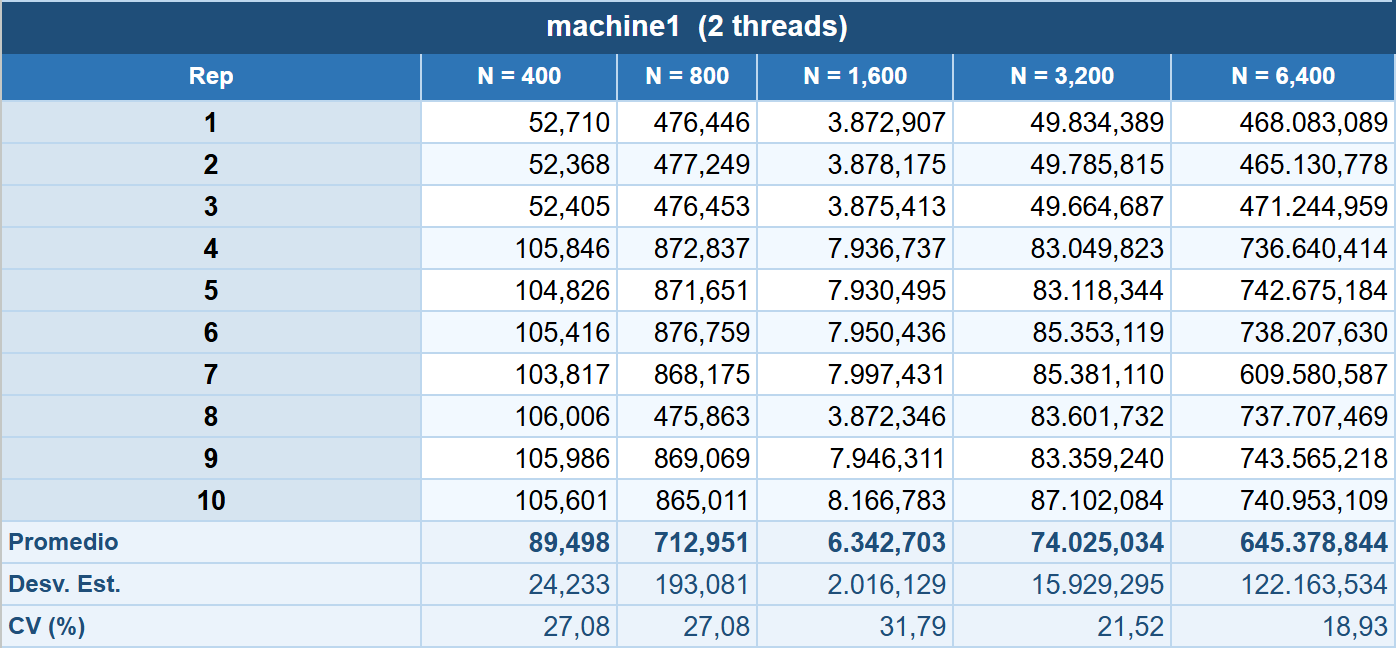
\includegraphics[width=1\textwidth]{images/omp/tables/time_machine1_2t.png}
   \caption{Resultados de tiempo para la multiplicación de matrices utilizando OpenMP con 2 hilos}
   \label{tab:time_machine1_2_threads}
\end{table}


\subsubsection{Pruebas con 4 hilos}
\label{sec:Pruebas con 4 hilos}

\begin{table}[H]
   \centering
   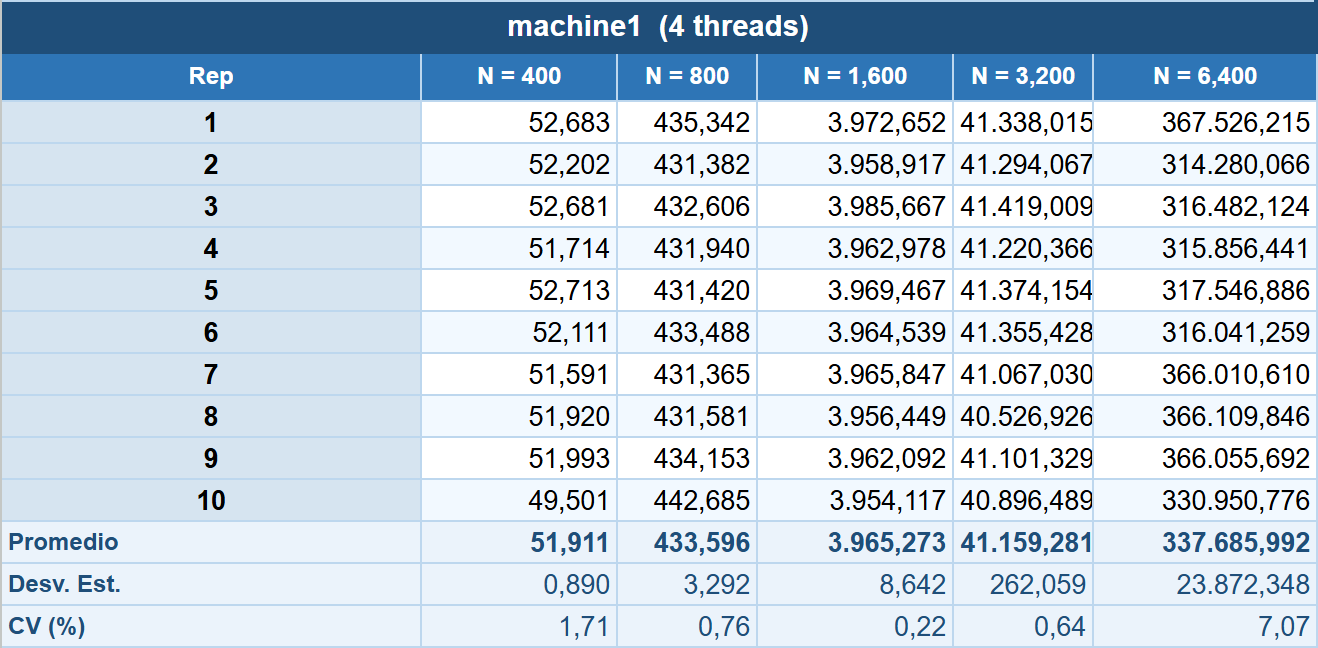
\includegraphics[width=1\textwidth]{images/omp/tables/time_machine1_4t.png}
   \caption{Resultados de tiempo para la multiplicación de matrices utilizando OpenMP con 4 hilos}
   \label{tab:time_machine1_4_threads}
\end{table}


%================================
\subsubsection{Pruebas con 6 hilos}
\label{sec:Pruebas con 6 hilos}

\begin{table}[H]
   \centering
   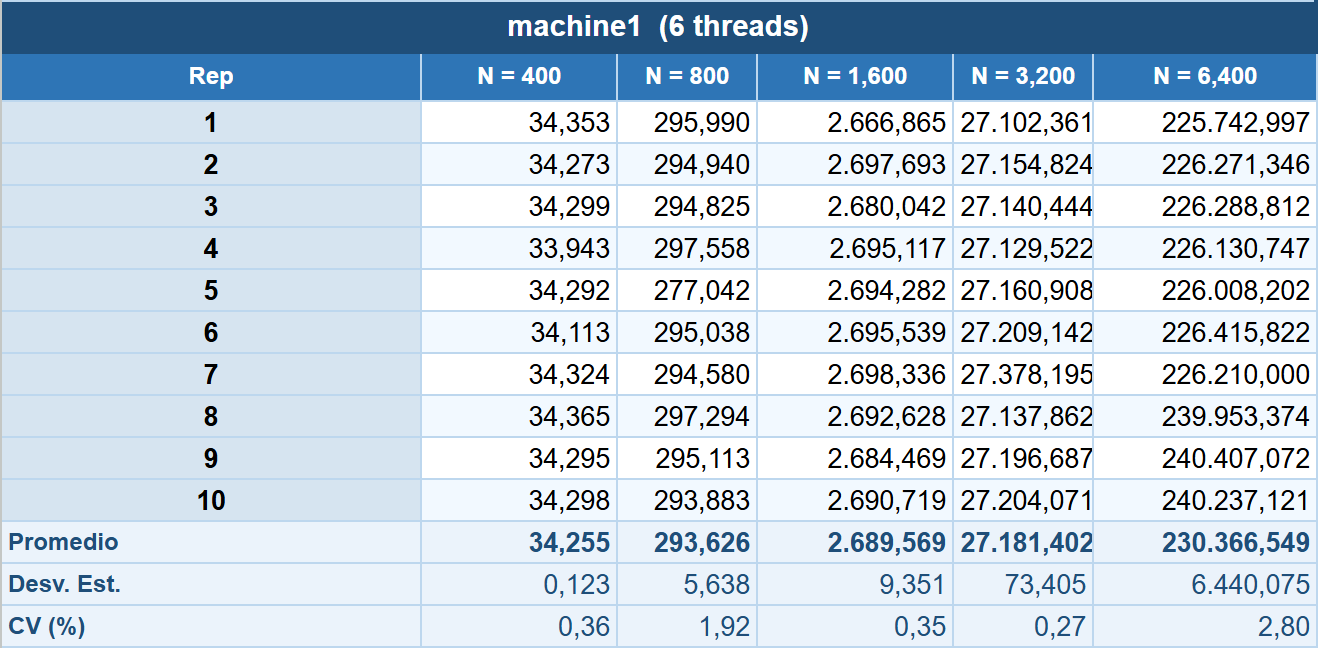
\includegraphics[width=1\textwidth]{images/omp/tables/time_machine1_6t.png}
   \caption{Resultados de tiempo para la multiplicación de matrices utilizando OpenMP con 6 hilos}
   \label{tab:time_machine1_6_threads}
\end{table}


\subsubsection{Pruebas con 8 hilos}
\label{sec:Pruebas con 8 hilos}

\begin{table}[H]
   \centering
   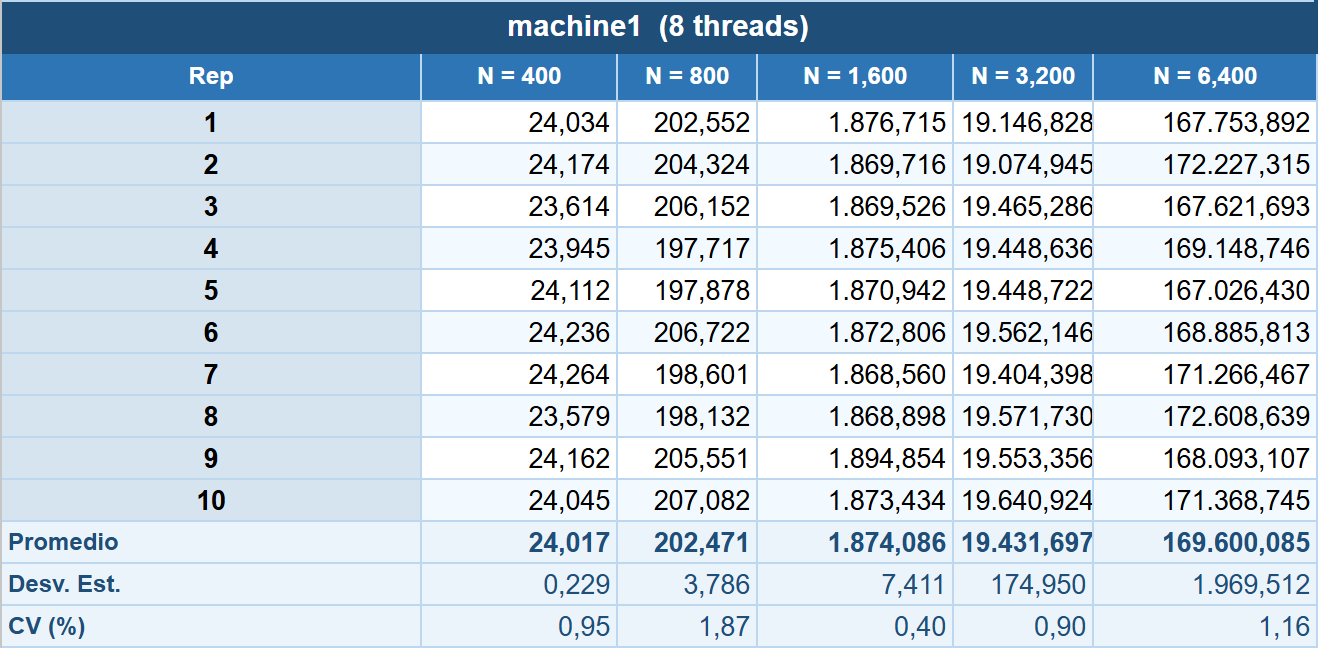
\includegraphics[width=1\textwidth]{images/omp/tables/time_machine1_8t.png}
   \caption{Resultados de tiempo para la multiplicación de matrices utilizando OpenMP con 8 hilos}
   \label{tab:time_machine1_8_threads}
\end{table}

\subsubsection{Pruebas con 12 hilos}
\label{sec:Pruebas con 12 hilos}

\begin{table}[H]
   \centering
   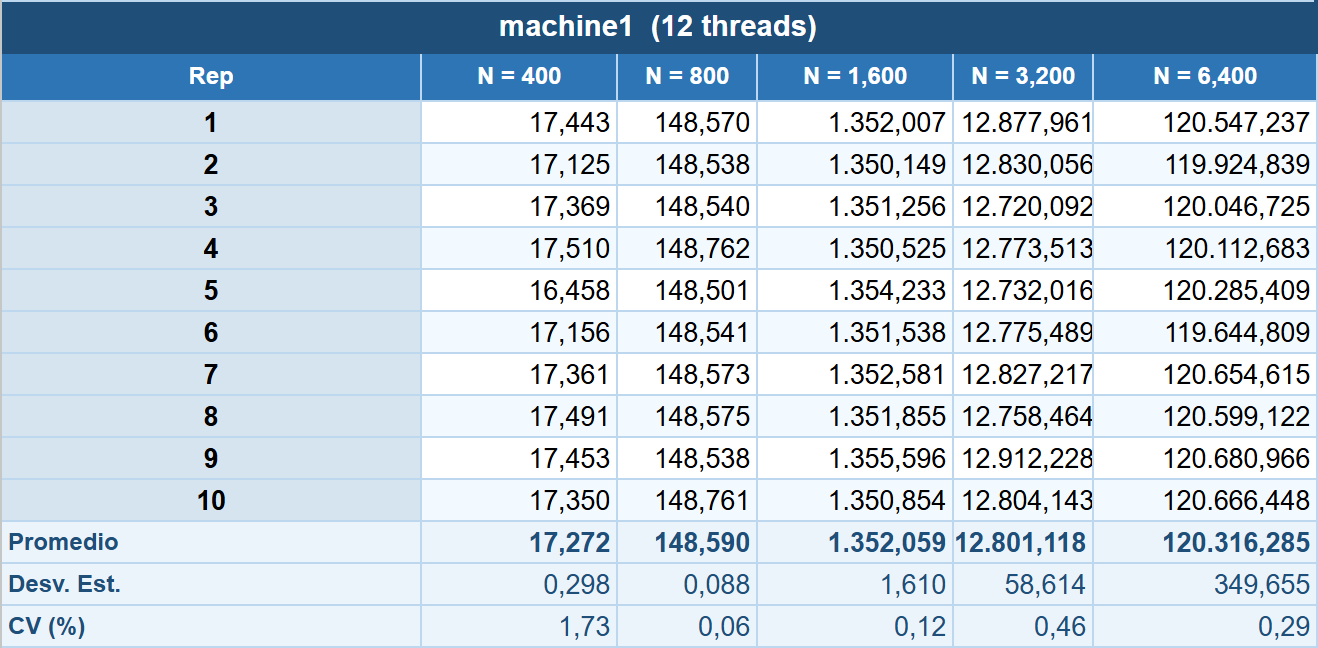
\includegraphics[width=1\textwidth]{images/omp/tables/time_machine1_12t.png}
   \caption{Resultados de tiempo para la multiplicación de matrices utilizando OpenMP con 12 hilos}
   \label{tab:time_machine1_12_threads}
\end{table}


\subsubsection{Gráfica tiempo de ejecución}
\label{sec:Gráfica tiempo de ejecución}

\begin{figure}[H]
   \centering
   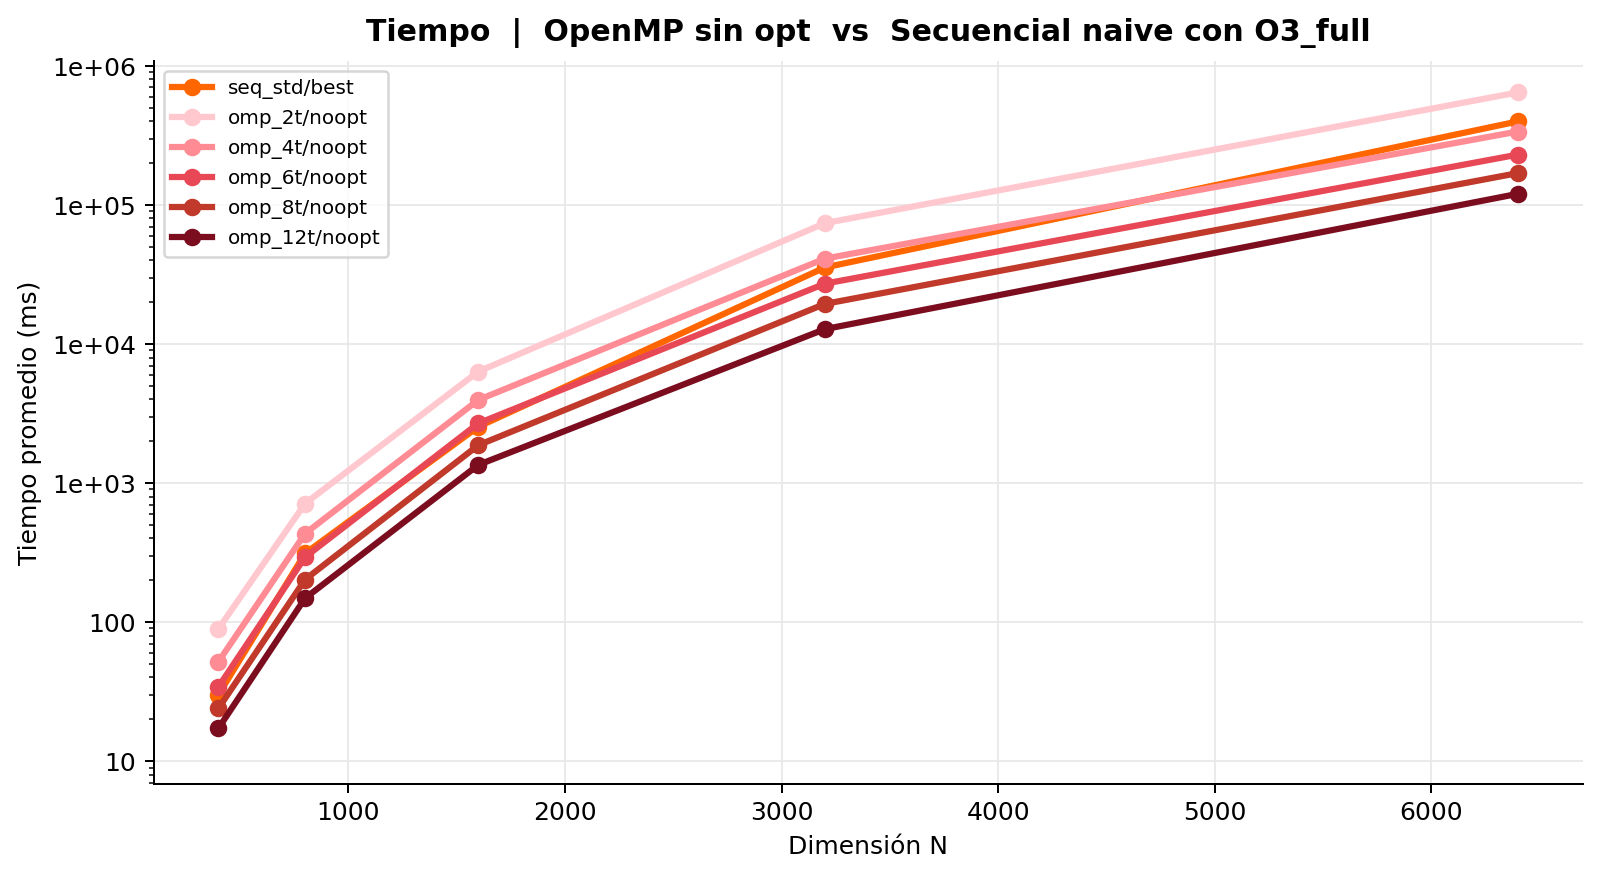
\includegraphics[width=1\textwidth]{images/omp/charts/time_omp_noopt.png}
   \caption{Gráfica de tiempo de ejecución para la multiplicación de matrices utilizando OpenMP sin optimización por compilador}
\end{figure}


%================================
\subsubsection{Speedup con OpenMP sin optimización}
\label{sec:Speedup con OpenMP}

\begin{table}[H]
   \centering
   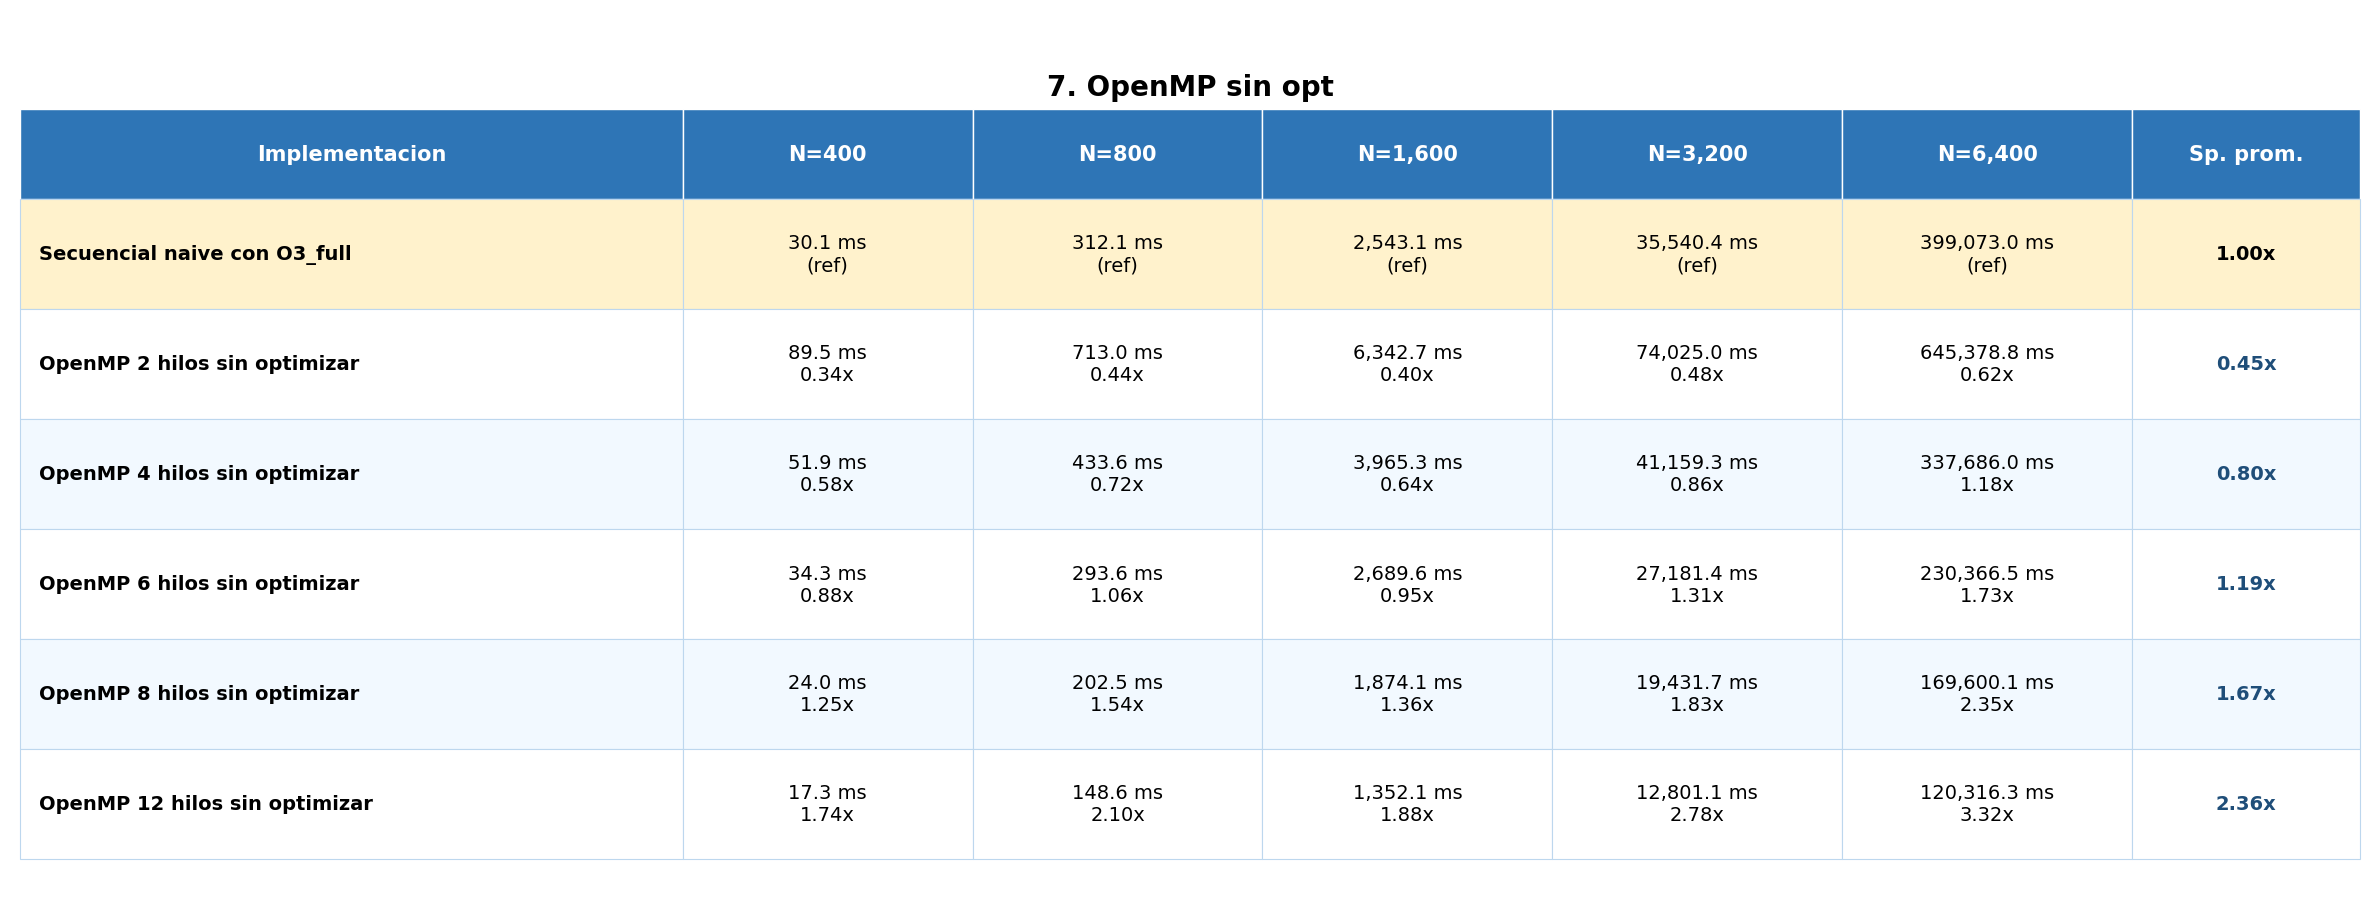
\includegraphics[width=1\textwidth]{images/omp/tables/table_noopt_speedup.png}
   \caption{Resultados de Speedup para la multiplicación de matrices utilizando OpenMP}
   \label{tab:speedup_machine1}
\end{table}

\begin{figure}[H]
   \centering
   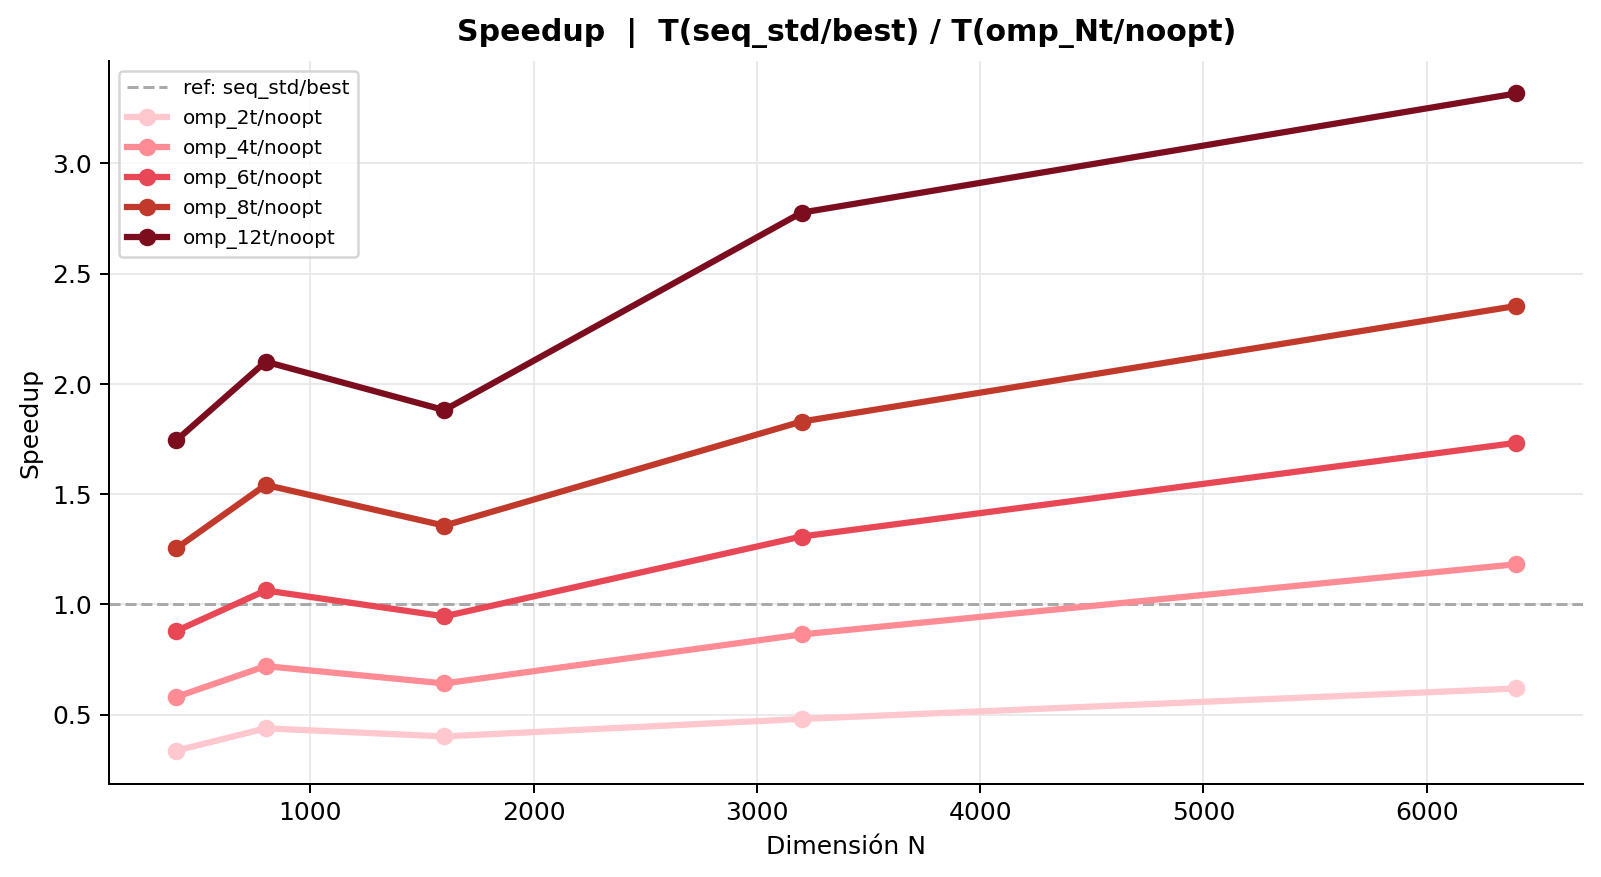
\includegraphics[width=1\textwidth]{images/omp/charts/speedup_omp_noopt.png}
   \caption{Gráfica de Speedup para la multiplicación de matrices utilizando OpenMP sin optimización}
\end{figure}


Como se ve en los resultados, entre más hilos se utilicen, el tiempo de ejecución disminuye, aunque no de manera lineal. Esto se debe a que la multiplicación de matrices es una tarea que se puede paralelizar, pero también tiene una parte secuencial que limita el speedup máximo que se puede alcanzar. Además, el overhead de crear y gestionar los hilos también puede afectar el rendimiento, especialmente cuando se utilizan muchos hilos. En este caso, vemos como OpenMP con 12 hilos tiene un speedup de 2.36x en comparación con la versión secuencial, siendo el más rápido en estas pruebas.